\subsection{Description of Data}

Table \ref{table:summaryStat_baseline} presents summary statistics for baseline variables by cohort and city. As mentioned above, certain baseline variables are missing for the adult cohorts due to differences in questionnaires administered to adults and children. The table illustrates differences and similarities in parental, caregiver and family characteristics across cities as well as over time. \textbf{[JJH: What is CAPI?]}

\begin{landscape}
\singlespace
\setlength{\tabcolsep}{2pt}
\begin{center}
\scriptsize{
\begin{longtable}{L{6cm} c c c p{.5cm} c c c p{.5cm} c c c p{.5cm} c c c p{.5cm} c c c}
\hline\multicolumn{20}{L{24cm}}{\textbf{Note:} Means are reported for each variable by cohort and city. Standard Deviations are reported in italics below each mean estimate. A . denotes that the variable is not defined for a specific cohort.}
\endfoot
\caption{Summary statistics for baseline variables by cohort and city} \label{table:summaryStat_baseline} \\
\hline
& \multicolumn{3}{c}{\textbf{Children}} & & \multicolumn{3}{c}{\textbf{Adolescents}} & & \multicolumn{3}{c}{\textbf{Adults 30}} & & \multicolumn{3}{c}{\textbf{Adults 40}} & & \multicolumn{3}{c}{\textbf{Adults 50}}\\
& \scriptsize{Reggio} & \scriptsize{Parma}& \scriptsize{Padova} & & \scriptsize{Reggio} & \scriptsize{Parma}& \scriptsize{Padova} & & \scriptsize{Reggio} & \scriptsize{Parma}& \scriptsize{Padova} & & \scriptsize{Reggio} & \scriptsize{Parma}& \scriptsize{Padova} & & \scriptsize{Reggio} & \scriptsize{Parma}& \scriptsize{Padova}\\
\hline \\[.2em] \endhead
 \quad Male & 0.54 &      0.56 &      0.52 & &      0.43 &      0.44 &      0.48 & &      0.60 &      0.53 &      0.55 & &      0.54 &      0.49 &      0.48 & &      0.47 &      0.38 &      0.46 \\*
 \quad & $\mathit{     0.50}$ & $\mathit{     0.50}$ & $\mathit{     0.50}$ & & $\mathit{     0.50}$ & $\mathit{     0.50}$ & $\mathit{     0.50}$ & & $\mathit{     0.49}$ & $\mathit{     0.50}$ & $\mathit{     0.50}$ & & $\mathit{     0.50}$ & $\mathit{     0.50}$ & $\mathit{     0.50}$ & & $\mathit{     0.50}$ & $\mathit{     0.49}$ & $\mathit{     0.50}$ \\[.2em]
 \quad Low birthweight & 0.08 &      0.07 &      0.05 & &      0.05 &      0.06 &      0.05 & &         . &         . &         . & &         . &         . &         . & &         . &         . &         . \\*
 \quad & $\mathit{     0.27}$ & $\mathit{     0.25}$ & $\mathit{     0.21}$ & & $\mathit{     0.23}$ & $\mathit{     0.24}$ & $\mathit{     0.21}$ & & $\mathit{        .}$ & $\mathit{        .}$ & $\mathit{        .}$ & & $\mathit{        .}$ & $\mathit{        .}$ & $\mathit{        .}$ & & $\mathit{        .}$ & $\mathit{        .}$ & $\mathit{        .}$ \\[.2em]
 \quad Premature birth & 0.10 &      0.08 &      0.07 & &      0.06 &      0.10 &      0.07 & &         . &         . &         . & &         . &         . &         . & &         . &         . &         . \\*
 \quad & $\mathit{     0.30}$ & $\mathit{     0.26}$ & $\mathit{     0.25}$ & & $\mathit{     0.24}$ & $\mathit{     0.30}$ & $\mathit{     0.25}$ & & $\mathit{        .}$ & $\mathit{        .}$ & $\mathit{        .}$ & & $\mathit{        .}$ & $\mathit{        .}$ & $\mathit{        .}$ & & $\mathit{        .}$ & $\mathit{        .}$ & $\mathit{        .}$ \\[.2em]
 \quad CAPI & 0.55 &      0.43 &      0.47 & &      0.43 &      0.55 &      0.49 & &      0.57 &      0.40 &      0.35 & &      0.63 &      0.34 &      0.35 & &      0.45 &      0.35 &      0.28 \\*
 \quad & $\mathit{     0.50}$ & $\mathit{     0.50}$ & $\mathit{     0.50}$ & & $\mathit{     0.50}$ & $\mathit{     0.50}$ & $\mathit{     0.50}$ & & $\mathit{     0.50}$ & $\mathit{     0.49}$ & $\mathit{     0.48}$ & & $\mathit{     0.48}$ & $\mathit{     0.48}$ & $\mathit{     0.48}$ & & $\mathit{     0.50}$ & $\mathit{     0.48}$ & $\mathit{     0.45}$ \\[.2em]
 \quad Born to teenaged mother & 0.00 &      0.01 &      0.01 & &      0.01 &      0.02 &      0.00 & &      1.00 &      1.00 &      1.00 & &      1.00 &      1.00 &      1.00 & &      1.00 &      1.00 &      1.00 \\*
 \quad & $\mathit{     0.00}$ & $\mathit{     0.08}$ & $\mathit{     0.08}$ & & $\mathit{     0.11}$ & $\mathit{     0.12}$ & $\mathit{     0.00}$ & & $\mathit{     0.00}$ & $\mathit{     0.00}$ & $\mathit{     0.00}$ & & $\mathit{     0.00}$ & $\mathit{     0.00}$ & $\mathit{     0.00}$ & & $\mathit{     0.00}$ & $\mathit{     0.00}$ & $\mathit{     0.00}$ \\[.2em]
 \quad Mom born in province & 0.51 &      0.60 &      0.69 & &      0.68 &      0.68 &      0.78 & &      0.84 &      0.70 &      0.71 & &      0.80 &      0.74 &      0.63 & &      0.78 &      0.80 &      0.76 \\*
 \quad & $\mathit{     0.50}$ & $\mathit{     0.49}$ & $\mathit{     0.46}$ & & $\mathit{     0.47}$ & $\mathit{     0.47}$ & $\mathit{     0.41}$ & & $\mathit{     0.36}$ & $\mathit{     0.46}$ & $\mathit{     0.46}$ & & $\mathit{     0.40}$ & $\mathit{     0.44}$ & $\mathit{     0.48}$ & & $\mathit{     0.42}$ & $\mathit{     0.40}$ & $\mathit{     0.43}$ \\[.2em]
 \quad Mom Max Edu: Low & 0.17 &      0.07 &      0.10 & &      0.16 &      0.11 &      0.14 & &      0.00 &      0.00 &      0.00 & &      0.02 &      0.00 &      0.00 & &      0.01 &      0.04 &      0.01 \\*
 \quad & $\mathit{     0.38}$ & $\mathit{     0.25}$ & $\mathit{     0.30}$ & & $\mathit{     0.36}$ & $\mathit{     0.31}$ & $\mathit{     0.35}$ & & $\mathit{     0.06}$ & $\mathit{     0.00}$ & $\mathit{     0.00}$ & & $\mathit{     0.13}$ & $\mathit{     0.00}$ & $\mathit{     0.06}$ & & $\mathit{     0.10}$ & $\mathit{     0.19}$ & $\mathit{     0.12}$ \\[.2em]
 \quad Mom Max Edu: Middle School & 0.08 &      0.05 &      0.09 & &      0.09 &      0.10 &      0.11 & &      0.03 &      0.07 &      0.10 & &      0.19 &      0.24 &      0.23 & &      0.41 &      0.55 &      0.64 \\*
 \quad & $\mathit{     0.27}$ & $\mathit{     0.23}$ & $\mathit{     0.29}$ & & $\mathit{     0.29}$ & $\mathit{     0.30}$ & $\mathit{     0.31}$ & & $\mathit{     0.18}$ & $\mathit{     0.25}$ & $\mathit{     0.30}$ & & $\mathit{     0.39}$ & $\mathit{     0.43}$ & $\mathit{     0.42}$ & & $\mathit{     0.49}$ & $\mathit{     0.50}$ & $\mathit{     0.48}$ \\[.2em]
 \quad Mom Max Edu: High School & 0.45 &      0.41 &      0.45 & &      0.48 &      0.44 &      0.43 & &      0.42 &      0.30 &      0.35 & &      0.47 &      0.35 &      0.35 & &      0.36 &      0.26 &      0.18 \\*
 \quad & $\mathit{     0.50}$ & $\mathit{     0.49}$ & $\mathit{     0.50}$ & & $\mathit{     0.50}$ & $\mathit{     0.50}$ & $\mathit{     0.50}$ & & $\mathit{     0.49}$ & $\mathit{     0.46}$ & $\mathit{     0.48}$ & & $\mathit{     0.50}$ & $\mathit{     0.48}$ & $\mathit{     0.48}$ & & $\mathit{     0.48}$ & $\mathit{     0.44}$ & $\mathit{     0.39}$ \\[.2em]
 \quad Mom Max Edu: University & 0.28 &      0.46 &      0.36 & &      0.25 &      0.33 &      0.29 & &      0.55 &      0.63 &      0.54 & &      0.31 &      0.41 &      0.41 & &      0.22 &      0.15 &      0.15 \\*
 \quad & $\mathit{     0.45}$ & $\mathit{     0.50}$ & $\mathit{     0.48}$ & & $\mathit{     0.43}$ & $\mathit{     0.47}$ & $\mathit{     0.46}$ & & $\mathit{     0.50}$ & $\mathit{     0.48}$ & $\mathit{     0.50}$ & & $\mathit{     0.46}$ & $\mathit{     0.49}$ & $\mathit{     0.49}$ & & $\mathit{     0.42}$ & $\mathit{     0.35}$ & $\mathit{     0.36}$ \\[.2em]
 \quad Born to teenaged father & 0.00 &      0.00 &      0.01 & &      0.00 &      0.01 &      0.00 & &      1.00 &      1.00 &      1.00 & &      1.00 &      1.00 &      1.00 & &      1.00 &      1.00 &      1.00 \\*
 \quad & $\mathit{     0.00}$ & $\mathit{     0.06}$ & $\mathit{     0.08}$ & & $\mathit{     0.00}$ & $\mathit{     0.09}$ & $\mathit{     0.06}$ & & $\mathit{     0.00}$ & $\mathit{     0.00}$ & $\mathit{     0.00}$ & & $\mathit{     0.00}$ & $\mathit{     0.00}$ & $\mathit{     0.00}$ & & $\mathit{     0.00}$ & $\mathit{     0.00}$ & $\mathit{     0.00}$ \\[.2em]
 \quad Father born in province & 0.52 &      0.59 &      0.64 & &      0.58 &      0.61 &      0.73 & &      0.87 &      0.79 &      0.76 & &      0.78 &      0.85 &      0.73 & &      0.84 &      0.65 &      0.82 \\*
 \quad & $\mathit{     0.50}$ & $\mathit{     0.49}$ & $\mathit{     0.48}$ & & $\mathit{     0.49}$ & $\mathit{     0.49}$ & $\mathit{     0.44}$ & & $\mathit{     0.34}$ & $\mathit{     0.41}$ & $\mathit{     0.43}$ & & $\mathit{     0.42}$ & $\mathit{     0.36}$ & $\mathit{     0.44}$ & & $\mathit{     0.37}$ & $\mathit{     0.48}$ & $\mathit{     0.38}$ \\[.2em]
 \quad Dad Max Edu: Low & 0.23 &      0.12 &      0.09 & &      0.19 &      0.16 &      0.14 & &         . &         . &         . & &      0.02 &      0.00 &      0.00 & &      0.01 &      0.04 &      0.02 \\*
 \quad & $\mathit{     0.42}$ & $\mathit{     0.33}$ & $\mathit{     0.29}$ & & $\mathit{     0.40}$ & $\mathit{     0.37}$ & $\mathit{     0.35}$ & & $\mathit{        .}$ & $\mathit{        .}$ & $\mathit{        .}$ & & $\mathit{     0.14}$ & $\mathit{     0.06}$ & $\mathit{     0.06}$ & & $\mathit{     0.07}$ & $\mathit{     0.19}$ & $\mathit{     0.14}$ \\[.2em]
 \quad Dad Max Edu: Middle School & 0.08 &      0.10 &      0.09 & &      0.09 &      0.07 &      0.10 & &      0.03 &      0.08 &      0.10 & &      0.19 &      0.22 &      0.14 & &      0.35 &      0.55 &      0.52 \\*
 \quad & $\mathit{     0.27}$ & $\mathit{     0.30}$ & $\mathit{     0.28}$ & & $\mathit{     0.28}$ & $\mathit{     0.26}$ & $\mathit{     0.30}$ & & $\mathit{     0.17}$ & $\mathit{     0.27}$ & $\mathit{     0.30}$ & & $\mathit{     0.39}$ & $\mathit{     0.41}$ & $\mathit{     0.35}$ & & $\mathit{     0.48}$ & $\mathit{     0.50}$ & $\mathit{     0.50}$ \\[.2em]
 \quad Dad Max Edu: High School & 0.35 &      0.36 &      0.42 & &      0.40 &      0.36 &      0.39 & &      0.37 &      0.32 &      0.32 & &      0.45 &      0.33 &      0.27 & &      0.36 &      0.19 &      0.17 \\*
 \quad & $\mathit{     0.48}$ & $\mathit{     0.48}$ & $\mathit{     0.49}$ & & $\mathit{     0.49}$ & $\mathit{     0.48}$ & $\mathit{     0.49}$ & & $\mathit{     0.48}$ & $\mathit{     0.47}$ & $\mathit{     0.47}$ & & $\mathit{     0.50}$ & $\mathit{     0.47}$ & $\mathit{     0.44}$ & & $\mathit{     0.48}$ & $\mathit{     0.40}$ & $\mathit{     0.38}$ \\[.2em]
 \quad Dad Max Edu: University & 0.24 &      0.35 &      0.30 & &      0.19 &      0.26 &      0.28 & &      0.60 &      0.60 &      0.57 & &      0.33 &      0.45 &      0.58 & &      0.27 &      0.20 &      0.27 \\*
 \quad & $\mathit{     0.43}$ & $\mathit{     0.48}$ & $\mathit{     0.46}$ & & $\mathit{     0.39}$ & $\mathit{     0.44}$ & $\mathit{     0.45}$ & & $\mathit{     0.49}$ & $\mathit{     0.49}$ & $\mathit{     0.50}$ & & $\mathit{     0.47}$ & $\mathit{     0.50}$ & $\mathit{     0.49}$ & & $\mathit{     0.45}$ & $\mathit{     0.40}$ & $\mathit{     0.45}$ \\[.2em]
 \quad Has 1 sibling & 0.52 &      0.46 &      0.50 & &      0.52 &      0.46 &      0.55 & &      0.36 &      0.33 &      0.45 & &      0.36 &      0.38 &      0.35 & &      0.28 &      0.26 &      0.39 \\*
 \quad & $\mathit{     0.50}$ & $\mathit{     0.50}$ & $\mathit{     0.50}$ & & $\mathit{     0.50}$ & $\mathit{     0.50}$ & $\mathit{     0.50}$ & & $\mathit{     0.48}$ & $\mathit{     0.47}$ & $\mathit{     0.50}$ & & $\mathit{     0.48}$ & $\mathit{     0.49}$ & $\mathit{     0.48}$ & & $\mathit{     0.45}$ & $\mathit{     0.44}$ & $\mathit{     0.49}$ \\[.2em]
 \quad Has 2 siblings & 0.14 &      0.21 &      0.17 & &      0.18 &      0.20 &      0.15 & &      0.24 &      0.33 &      0.25 & &      0.27 &      0.33 &      0.35 & &      0.30 &      0.27 &      0.22 \\*
 \quad & $\mathit{     0.35}$ & $\mathit{     0.41}$ & $\mathit{     0.37}$ & & $\mathit{     0.38}$ & $\mathit{     0.40}$ & $\mathit{     0.36}$ & & $\mathit{     0.43}$ & $\mathit{     0.47}$ & $\mathit{     0.43}$ & & $\mathit{     0.44}$ & $\mathit{     0.47}$ & $\mathit{     0.48}$ & & $\mathit{     0.46}$ & $\mathit{     0.45}$ & $\mathit{     0.42}$ \\[.2em]
 \quad Has more than 2 siblings & 0.06 &      0.04 &      0.05 & &      0.09 &      0.06 &      0.02 & &      0.13 &      0.20 &      0.17 & &      0.20 &      0.19 &      0.26 & &      0.34 &      0.39 &      0.35 \\*
 \quad & $\mathit{     0.23}$ & $\mathit{     0.19}$ & $\mathit{     0.21}$ & & $\mathit{     0.29}$ & $\mathit{     0.24}$ & $\mathit{     0.16}$ & & $\mathit{     0.33}$ & $\mathit{     0.40}$ & $\mathit{     0.37}$ & & $\mathit{     0.40}$ & $\mathit{     0.39}$ & $\mathit{     0.44}$ & & $\mathit{     0.48}$ & $\mathit{     0.49}$ & $\mathit{     0.48}$ \\[.2em]
 \quad Caregiver was Catholic & 0.77 &      0.83 &      0.79 & &      0.75 &      0.86 &      0.73 & &         . &         . &         . & &         . &         . &         . & &         . &         . &         . \\*
 \quad & $\mathit{     0.42}$ & $\mathit{     0.37}$ & $\mathit{     0.41}$ & & $\mathit{     0.43}$ & $\mathit{     0.35}$ & $\mathit{     0.44}$ & & $\mathit{        .}$ & $\mathit{        .}$ & $\mathit{        .}$ & & $\mathit{        .}$ & $\mathit{        .}$ & $\mathit{        .}$ & & $\mathit{        .}$ & $\mathit{        .}$ & $\mathit{        .}$ \\[.2em]
 \quad Caregiver was faithful and Catholic & 0.47 &      0.52 &      0.51 & &      0.45 &      0.54 &      0.45 & &         . &         . &         . & &         . &         . &         . & &         . &         . &         . \\*
 \quad & $\mathit{     0.50}$ & $\mathit{     0.50}$ & $\mathit{     0.50}$ & & $\mathit{     0.50}$ & $\mathit{     0.50}$ & $\mathit{     0.50}$ & & $\mathit{        .}$ & $\mathit{        .}$ & $\mathit{        .}$ & & $\mathit{        .}$ & $\mathit{        .}$ & $\mathit{        .}$ & & $\mathit{        .}$ & $\mathit{        .}$ & $\mathit{        .}$ \\[.2em]
 \quad Caregiver owned house & 0.58 &      0.71 &      0.66 & &      0.84 &      0.81 &      0.77 & &         . &         . &         . & &         . &         . &         . & &         . &         . &         . \\*
 \quad & $\mathit{     0.49}$ & $\mathit{     0.46}$ & $\mathit{     0.48}$ & & $\mathit{     0.37}$ & $\mathit{     0.39}$ & $\mathit{     0.42}$ & & $\mathit{        .}$ & $\mathit{        .}$ & $\mathit{        .}$ & & $\mathit{        .}$ & $\mathit{        .}$ & $\mathit{        .}$ & & $\mathit{        .}$ & $\mathit{        .}$ & $\mathit{        .}$ \\[.2em]
 \quad Caregiver was a migrant & 0.07 &      0.02 &      0.02 & &      0.01 &      0.02 &      0.00 & &         . &         . &         . & &         . &         . &         . & &         . &         . &         . \\*
 \quad & $\mathit{     0.26}$ & $\mathit{     0.14}$ & $\mathit{     0.15}$ & & $\mathit{     0.11}$ & $\mathit{     0.12}$ & $\mathit{     0.00}$ & & $\mathit{        .}$ & $\mathit{        .}$ & $\mathit{        .}$ & & $\mathit{        .}$ & $\mathit{        .}$ & $\mathit{        .}$ & & $\mathit{        .}$ & $\mathit{        .}$ & $\mathit{        .}$ \\[.2em]
 \quad Caregiver Income: 5,000 euros or less & 0.01 &      0.02 &      0.03 & &      0.00 &      0.02 &      0.04 & &         . &         . &         . & &         . &         . &         . & &         . &         . &         . \\*
 \quad & $\mathit{     0.11}$ & $\mathit{     0.15}$ & $\mathit{     0.18}$ & & $\mathit{     0.06}$ & $\mathit{     0.15}$ & $\mathit{     0.19}$ & & $\mathit{        .}$ & $\mathit{        .}$ & $\mathit{        .}$ & & $\mathit{        .}$ & $\mathit{        .}$ & $\mathit{        .}$ & & $\mathit{        .}$ & $\mathit{        .}$ & $\mathit{        .}$ \\[.2em]
 \quad Caregiver Income: 5,001-10,000 euros & 0.01 &      0.02 &      0.01 & &      0.01 &      0.01 &      0.01 & &         . &         . &         . & &         . &         . &         . & &         . &         . &         . \\*
 \quad & $\mathit{     0.11}$ & $\mathit{     0.13}$ & $\mathit{     0.12}$ & & $\mathit{     0.10}$ & $\mathit{     0.09}$ & $\mathit{     0.08}$ & & $\mathit{        .}$ & $\mathit{        .}$ & $\mathit{        .}$ & & $\mathit{        .}$ & $\mathit{        .}$ & $\mathit{        .}$ & & $\mathit{        .}$ & $\mathit{        .}$ & $\mathit{        .}$ \\[.2em]
 \quad Caregiver Income: 10,001-25,000 euros & 0.17 &      0.19 &      0.15 & &      0.18 &      0.18 &      0.10 & &         . &         . &         . & &         . &         . &         . & &         . &         . &         . \\*
 \quad & $\mathit{     0.38}$ & $\mathit{     0.39}$ & $\mathit{     0.36}$ & & $\mathit{     0.39}$ & $\mathit{     0.38}$ & $\mathit{     0.30}$ & & $\mathit{        .}$ & $\mathit{        .}$ & $\mathit{        .}$ & & $\mathit{        .}$ & $\mathit{        .}$ & $\mathit{        .}$ & & $\mathit{        .}$ & $\mathit{        .}$ & $\mathit{        .}$ \\[.2em]
 \quad Caregiver Income: 25,001-50,000 euros & 0.32 &      0.41 &      0.32 & &      0.32 &      0.29 &      0.24 & &         . &         . &         . & &         . &         . &         . & &         . &         . &         . \\*
 \quad & $\mathit{     0.47}$ & $\mathit{     0.49}$ & $\mathit{     0.47}$ & & $\mathit{     0.47}$ & $\mathit{     0.46}$ & $\mathit{     0.43}$ & & $\mathit{        .}$ & $\mathit{        .}$ & $\mathit{        .}$ & & $\mathit{        .}$ & $\mathit{        .}$ & $\mathit{        .}$ & & $\mathit{        .}$ & $\mathit{        .}$ & $\mathit{        .}$ \\[.2em]
 \quad Caregiver Income: 50,001-100,000 euros & 0.19 &      0.19 &      0.13 & &      0.24 &      0.24 &      0.11 & &         . &         . &         . & &         . &         . &         . & &         . &         . &         . \\*
 \quad & $\mathit{     0.40}$ & $\mathit{     0.39}$ & $\mathit{     0.34}$ & & $\mathit{     0.43}$ & $\mathit{     0.43}$ & $\mathit{     0.31}$ & & $\mathit{        .}$ & $\mathit{        .}$ & $\mathit{        .}$ & & $\mathit{        .}$ & $\mathit{        .}$ & $\mathit{        .}$ & & $\mathit{        .}$ & $\mathit{        .}$ & $\mathit{        .}$ \\[.2em]
 \quad Caregiver Income: 100,001-250,000 euros & 0.02 &      0.02 &      0.03 & &      0.04 &      0.03 &      0.02 & &         . &         . &         . & &         . &         . &         . & &         . &         . &         . \\*
 \quad & $\mathit{     0.15}$ & $\mathit{     0.14}$ & $\mathit{     0.17}$ & & $\mathit{     0.20}$ & $\mathit{     0.17}$ & $\mathit{     0.16}$ & & $\mathit{        .}$ & $\mathit{        .}$ & $\mathit{        .}$ & & $\mathit{        .}$ & $\mathit{        .}$ & $\mathit{        .}$ & & $\mathit{        .}$ & $\mathit{        .}$ & $\mathit{        .}$ \\[.2em]
 \quad Caregiver Income: > 250,000 euros & . &         . &         . & &      0.00 &      0.00 &      0.00 & &         . &         . &         . & &         . &         . &         . & &         . &         . &         . \\*
 \quad & $\mathit{        .}$ & $\mathit{        .}$ & $\mathit{        .}$ & & $\mathit{     0.06}$ & $\mathit{     0.00}$ & $\mathit{     0.00}$ & & $\mathit{        .}$ & $\mathit{        .}$ & $\mathit{        .}$ & & $\mathit{        .}$ & $\mathit{        .}$ & $\mathit{        .}$ & & $\mathit{        .}$ & $\mathit{        .}$ & $\mathit{        .}$ \\[.2em]
 \quad Caregiver was religious & 0.85 &      0.87 &      0.80 & &      0.77 &      0.87 &      0.74 & &      0.50 &      0.73 &      0.72 & &      0.50 &      0.75 &      0.75 & &      0.64 &      0.71 &      0.77 \\*
 \quad & $\mathit{     0.36}$ & $\mathit{     0.34}$ & $\mathit{     0.40}$ & & $\mathit{     0.42}$ & $\mathit{     0.34}$ & $\mathit{     0.44}$ & & $\mathit{     0.50}$ & $\mathit{     0.45}$ & $\mathit{     0.45}$ & & $\mathit{     0.50}$ & $\mathit{     0.43}$ & $\mathit{     0.44}$ & & $\mathit{     0.48}$ & $\mathit{     0.46}$ & $\mathit{     0.42}$ \\[.2em]
 ~\\[-.5em]
\hline
\end{longtable}
}
\end{center}

\end{landscape}

\subsection{Characteristics of Reggio Emilia, Parma, and Padova}
\label{app:characteristics-cities}

Table~\ref{table:data-sources} lists the sources of the myriad of historical records that we investigated. Tables~\ref{table:demo-employ} and~\ref{table:demo-other} describe the cities along demographic characteristics based on those records. Reggio Emilia and Parma, in addition to being geographically close are socially and economically similar.

\begin{table}[H]
\centering
\footnotesize
	\caption{Summary of Data Sources} \label{table:data-sources}
	\begin{tabular}{lll}
\toprule
\multicolumn{1}{c}{Type}	&	\multicolumn{1}{c}{Variables}	&	\multicolumn{1}{c}{Sources}	\\
\midrule
			&	Population & \\
			& 	Age distribution & \\
			&	Aging index & \\
Census Data	&	Marital status & \citet{Istat_2014_Atlante-Statistico} \\
			& 	Educational attainment & \\
			& 	Economic activity & \\
			& 	Employment by industry & \\
			& 	Homeownership	&	\\
\midrule
						&		Birth rates 			&	\citet{Reggio-Emilia-Admin-Data_1966-2010}, \\
						&	Mortality rates		& 	\citet{Padova-Admin-Data_1964-2010}, 	\\
	Demographic Statistics	&	 Internal migration 		&	\citet{Statistica-Regionae_2016_Veneto}, \\
						&	Foreign migration 	&  	\citet{Emilia-Romagna_2016_Population},\\
						&	Married in religious ceremonies		&	and \citet{Istat_2016_Geo-Demo} \\
\midrule
						&	School-level preschool enrollment	 &	\citet{Reggio-Annual-Journals_1994-2011}, \\
	Early Education Statistics	& 	School-level infant-toddler enrollment & 	\citet{Padova-Admin-Data_1964-2010},  \\
						& 	Child-teacher ratios				&	and \citet{Reggio-Emilia-Admin-Data_1966-2010} \\
\midrule
Election Data				&	\% of Votes to PCI and DC parties 	&	\citet{Archivo-Storico_2016} \\
\bottomrule
\end{tabular}


\end{table}


\begin{landscape}
\begin{table}[ht!]
\begin{center}
\scriptsize{
	\caption{Proportion of Individuals in Different Employment and Industry Categories} \label{table:demo-employ}
	
\begin{tabular}{L{6.5cm} *{3}{*{5}{c} c}}
\hline \\[-7pt]
& \multicolumn{5}{c}{\textbf{Reggio Emilia}} & & \multicolumn{5}{c}{\textbf{Parma}} & & \multicolumn{5}{c}{\textbf{Padova}} \\[3pt]
& \textbf{1971} & \textbf{1981} & \textbf{1991} & \textbf{2001} & \textbf{2011} & & \textbf{1971} & \textbf{1981} & \textbf{1991} & \textbf{2001} & \textbf{2011} & & \textbf{1971} & \textbf{1981} & \textbf{1991} & \textbf{2001} & \textbf{2011} \\[3pt]
\hline \\
\textbf{Employment}\\
\quad Employed (B) & 0.48 & 0.51 & 0.49 & 0.53 & 0.53 & & 0.47 & 0.49 & 0.49 & 0.50 & 0.53 & & 0.45 & 0.46 & 0.45 & 0.47 & 0.49 & \\ 
\quad Employed (F) & 0.28 & 0.37 & 0.38 & 0.43 & 0.46 & & 0.26 & 0.34 & 0.37 & 0.41 & 0.46 & & 0.24 & 0.30 & 0.32 & 0.37 & 0.42 & \\ 
\quad Employed (M) & 0.70 & 0.66 & 0.61 & 0.63 & 0.62 & & 0.70 & 0.66 & 0.62 & 0.60 & 0.60 & & 0.69 & 0.64 & 0.60 & 0.59 & 0.57 & \\[5pt] 
\quad Unemployed (B) & 0.01 & 0.01 & 0.02 & 0.02 & 0.06 & & 0.02 & 0.02 & 0.01 & 0.02 & 0.03 & & 0.02 & 0.01 & 0.02 & 0.03 & 0.04 & \\ 
\quad Unemployed (F) & 0.01 & 0.01 & 0.02 & 0.03 & 0.06 & & 0.01 & 0.02 & 0.01 & 0.02 & 0.03 & & 0.01 & 0.01 & 0.02 & 0.03 & 0.04 & \\ 
\quad Unemployed (M) & 0.02 & 0.01 & 0.02 & 0.02 & 0.05 & & 0.02 & 0.01 & 0.01 & 0.02 & 0.03 & & 0.02 & 0.02 & 0.03 & 0.03 & 0.04 & \\[5pt] 
\quad Homemaker (B) & 0.26 & 0.17 & 0.13 & 0.11 & 0.06 & & 0.28 & 0.20 & 0.16 & 0.12 & 0.07 & & 0.32 & 0.25 & 0.21 & 0.16 & 0.09 & \\ 
\quad Homemaker (F) & 0.50 & 0.33 & 0.25 & 0.20 & 0.11 & & 0.53 & 0.37 & 0.30 & 0.22 & 0.12 & & 0.59 & 0.47 & 0.38 & 0.30 & 0.16 & \\ 
\quad Homemaker (M) & 0.00 & 0.00 & 0.00 & 0.00 & 0.00 & & 0.00 & 0.00 & 0.00 & 0.00 & 0.00 & & 0.00 & 0.00 & 0.00 & 0.00 & 0.01 & \\[5pt] 
\quad Pensioner (B) & 0.15 & 0.21 & 0.23 & 0.24 & 0.25 & & 0.15 & 0.19 & 0.21 & 0.24 & 0.27 & & 0.11 & 0.13 & 0.16 & 0.21 & 0.26 & \\ 
\quad Pensioner (F) & 0.13 & 0.20 & 0.22 & 0.23 & 0.27 & & 0.13 & 0.17 & 0.19 & 0.22 & 0.28 & & 0.07 & 0.09 & 0.12 & 0.18 & 0.27 & \\ 
\quad Pensioner (M) & 0.17 & 0.22 & 0.24 & 0.25 & 0.23 & & 0.18 & 0.21 & 0.23 & 0.26 & 0.25 & & 0.15 & 0.17 & 0.20 & 0.26 & 0.25 & \\[5pt] 
\quad Student (B) & 0.07 & 0.07 & 0.08 & 0.06 & 0.06 & & 0.07 & 0.08 & 0.09 & 0.07 & 0.07 & & 0.09 & 0.11 & 0.11 & 0.08 & 0.08 & \\ 
\quad Student (F) & 0.06 & 0.07 & 0.08 & 0.05 & 0.06 & & 0.06 & 0.08 & 0.08 & 0.06 & 0.06 & & 0.07 & 0.10 & 0.10 & 0.07 & 0.07 & \\ 
\quad Student (M) & 0.08 & 0.08 & 0.08 & 0.06 & 0.07 & & 0.08 & 0.09 & 0.09 & 0.07 & 0.07 & & 0.11 & 0.13 & 0.12 & 0.08 & 0.08 & \\[5pt] 
\quad Other (B) & 0.03 & 0.03 & 0.05 & 0.05 & 0.04 & & 0.02 & 0.02 & 0.04 & 0.05 & 0.04 & & 0.02 & 0.03 & 0.05 & 0.05 & 0.05 & \\ 
\quad Other (F) & 0.03 & 0.02 & 0.05 & 0.05 & 0.04 & & 0.02 & 0.02 & 0.04 & 0.05 & 0.04 & & 0.02 & 0.02 & 0.05 & 0.05 & 0.04 & \\ 
\quad Other (M) & 0.04 & 0.03 & 0.04 & 0.04 & 0.04 & & 0.02 & 0.03 & 0.04 & 0.05 & 0.04 & & 0.03 & 0.04 & 0.05 & 0.05 & 0.05 & \\[5pt] 
\textbf{Industry}\\
\quad Agriculture, Forestry And Fishing (B) &   . & 0.08 & 0.04 & 0.04 & 0.04 & &   . & 0.05 & 0.02 & 0.02 & 0.03 & &   . & 0.01 & 0.01 & 0.01 & 0.01 & \\ 
\quad Agriculture, Forestry And Fishing (F) &   . & 0.06 & 0.03 & 0.03 & 0.02 & &   . & 0.04 & 0.01 & 0.02 & 0.02 & &   . & 0.01 & 0.01 & 0.01 & 0.01 & \\ 
\quad Agriculture, Forestry And Fishing (M) &   . & 0.10 & 0.05 & 0.04 & 0.05 & &   . & 0.05 & 0.03 & 0.03 & 0.04 & &   . & 0.02 & 0.01 & 0.01 & 0.02 & \\[5pt] 
\quad Finance, Professional, Scientific, Admin (B) &   . & 0.07 & 0.11 & 0.11 & 0.14 & &   . & 0.08 & 0.13 & 0.14 & 0.17 & &   . & 0.09 & 0.15 & 0.17 & 0.19 & \\ 
\quad Finance, Professional, Scientific, Admin (F) &   . & 0.06 & 0.12 & 0.12 & 0.15 & &   . & 0.07 & 0.15 & 0.14 & 0.18 & &   . & 0.08 & 0.15 & 0.17 & 0.19 & \\ 
\quad Finance, Professional, Scientific, Admin (M) &   . & 0.07 & 0.10 & 0.11 & 0.13 & &   . & 0.08 & 0.12 & 0.13 & 0.16 & &   . & 0.09 & 0.15 & 0.17 & 0.20 & \\[5pt] 
\quad Trade, Hotels And Restaurants  (B) &   . & 0.19 & 0.20 & 0.19 & 0.18 & &   . & 0.20 & 0.19 & 0.18 & 0.17 & &   . & 0.26 & 0.23 & 0.20 & 0.16 & \\ 
\quad Trade, Hotels And Restaurants  (F) &   . & 0.20 & 0.21 & 0.21 & 0.20 & &   . & 0.21 & 0.21 & 0.20 & 0.18 & &   . & 0.24 & 0.21 & 0.19 & 0.16 & \\ 
\quad Trade, Hotels And Restaurants  (M) &   . & 0.18 & 0.19 & 0.18 & 0.16 & &   . & 0.19 & 0.18 & 0.17 & 0.15 & &   . & 0.26 & 0.23 & 0.20 & 0.17 & \\[5pt] 
\quad Transport, Storage, Info, Communication  (B) &   . & 0.05 & 0.04 & 0.04 & 0.06 & &   . & 0.05 & 0.05 & 0.04 & 0.06 & &   . & 0.06 & 0.05 & 0.05 & 0.07 & \\ 
\quad Transport, Storage, Info, Communication  (F) &   . & 0.02 & 0.03 & 0.02 & 0.03 & &   . & 0.02 & 0.03 & 0.02 & 0.04 & &   . & 0.03 & 0.03 & 0.03 & 0.04 & \\ 
\quad Transport, Storage, Info, Communication  (M) &   . & 0.06 & 0.05 & 0.05 & 0.07 & &   . & 0.07 & 0.06 & 0.05 & 0.08 & &   . & 0.08 & 0.07 & 0.06 & 0.09 & \\[5pt] 
\quad Other Activities  (B) &   . & 0.24 & 0.23 & 0.25 & 0.28 & &   . & 0.25 & 0.25 & 0.28 & 0.31 & &   . & 0.32 & 0.32 & 0.35 & 0.37 & \\ 
\quad Other Activities  (F) &   . & 0.36 & 0.34 & 0.38 & 0.43 & &   . & 0.39 & 0.36 & 0.41 & 0.44 & &   . & 0.47 & 0.44 & 0.47 & 0.51 & \\ 
\quad Other Activities  (M) &   . & 0.16 & 0.16 & 0.15 & 0.15 & &   . & 0.17 & 0.18 & 0.19 & 0.20 & &   . & 0.24 & 0.25 & 0.27 & 0.25 & \\[5pt] 
\hline \\[-7pt]
\multicolumn{19}{L{24cm}}{\textbf{Note:} This table presents the percentage of individuals in different employment and industry categories within each city during each of the 5 listed years. Percentages are reported for females (F), males (M), and both genders (B) combined. The percentages are calculated using the total number of individuals above age 15 for the denominator. Data were collected from ISTAT and regional agencies.}
\end{tabular}

}
\end{center}
\end{table}
\end{landscape}

\begin{landscape}
\begin{table}[ht!]
\begin{center}
\scriptsize{
	\caption{Proportion of Individuals in Different Education, Rental, and Marital Categories} \label{table:demo-other}
	
\begin{tabular}{L{5cm} *{3}{*{5}{c} c}}
\hline \\[-7pt]
& \multicolumn{5}{c}{\textbf{Reggio Emilia}} & & \multicolumn{5}{c}{\textbf{Parma}} & & \multicolumn{5}{c}{\textbf{Padova}} \\[3pt]
& \textbf{1971} & \textbf{1981} & \textbf{1991} & \textbf{2001} & \textbf{2011} & & \textbf{1971} & \textbf{1981} & \textbf{1991} & \textbf{2001} & \textbf{2011} & & \textbf{1971} & \textbf{1981} & \textbf{1991} & \textbf{2001} & \textbf{2011} \\[3pt]
\hline \\
~\\[-4pt]
\textbf{Education}\\
\quad $<$ Primary (B) & 0.27 & 0.15 & 0.10 & 0.08 & 0.07 & & 0.28 & 0.14 & 0.09 & 0.07 & 0.06 & & 0.23 & 0.13 & 0.08 & 0.06 & 0.06 & \\ 
\quad $<$ Primary (F) & 0.31 & 0.17 & 0.11 & 0.09 & 0.08 & & 0.32 & 0.16 & 0.10 & 0.08 & 0.07 & & 0.26 & 0.14 & 0.09 & 0.07 & 0.06 & \\ 
\quad $<$ Primary (M) & 0.23 & 0.13 & 0.08 & 0.07 & 0.07 & & 0.23 & 0.12 & 0.07 & 0.06 & 0.06 & & 0.20 & 0.11 & 0.06 & 0.06 & 0.06 & \\[5pt] 
\quad Primary (B) & 0.45 & 0.43 & 0.34 & 0.26 & 0.18 & & 0.43 & 0.41 & 0.32 & 0.24 & 0.18 & & 0.41 & 0.35 & 0.27 & 0.21 & 0.17 & \\ 
\quad Primary (F) & 0.44 & 0.45 & 0.37 & 0.28 & 0.21 & & 0.42 & 0.43 & 0.35 & 0.27 & 0.20 & & 0.42 & 0.39 & 0.31 & 0.25 & 0.20 & \\ 
\quad Primary (M) & 0.46 & 0.40 & 0.31 & 0.22 & 0.16 & & 0.43 & 0.38 & 0.28 & 0.21 & 0.15 & & 0.39 & 0.31 & 0.22 & 0.17 & 0.13 & \\[5pt] 
\quad Lower Secondary (B) & 0.16 & 0.24 & 0.27 & 0.27 & 0.27 & & 0.16 & 0.24 & 0.28 & 0.25 & 0.25 & & 0.20 & 0.26 & 0.28 & 0.25 & 0.23 & \\ 
\quad Lower Secondary (F) & 0.14 & 0.21 & 0.23 & 0.23 & 0.24 & & 0.15 & 0.21 & 0.25 & 0.23 & 0.22 & & 0.19 & 0.24 & 0.26 & 0.23 & 0.21 & \\ 
\quad Lower Secondary (M) & 0.17 & 0.26 & 0.31 & 0.31 & 0.31 & & 0.18 & 0.26 & 0.31 & 0.28 & 0.27 & & 0.22 & 0.28 & 0.31 & 0.27 & 0.24 & \\[5pt] 
\quad High School (B) & 0.10 & 0.15 & 0.24 & 0.30 & 0.33 & & 0.10 & 0.16 & 0.24 & 0.30 & 0.32 & & 0.12 & 0.19 & 0.27 & 0.30 & 0.31 & \\ 
\quad High School (F) & 0.09 & 0.14 & 0.24 & 0.29 & 0.33 & & 0.09 & 0.16 & 0.24 & 0.29 & 0.31 & & 0.10 & 0.17 & 0.25 & 0.29 & 0.30 & \\ 
\quad High School (M) & 0.11 & 0.16 & 0.24 & 0.30 & 0.33 & & 0.11 & 0.17 & 0.25 & 0.31 & 0.33 & & 0.13 & 0.20 & 0.28 & 0.32 & 0.33 & \\[5pt] 
\quad Post Secondary Degree (B) & 0.02 & 0.04 & 0.06 & 0.10 & 0.14 & & 0.03 & 0.05 & 0.07 & 0.14 & 0.19 & & 0.04 & 0.07 & 0.11 & 0.17 & 0.24 & \\ 
\quad Post Secondary Degree (F) & 0.02 & 0.03 & 0.05 & 0.10 & 0.15 & & 0.02 & 0.04 & 0.06 & 0.13 & 0.20 & & 0.03 & 0.05 & 0.09 & 0.16 & 0.23 & \\ 
\quad Post Secondary Degree (M) & 0.03 & 0.05 & 0.07 & 0.10 & 0.13 & & 0.04 & 0.06 & 0.09 & 0.14 & 0.19 & & 0.06 & 0.09 & 0.13 & 0.19 & 0.24 & \\[5pt] 
~\\[-4pt]
\textbf{Rental Status}\\
%\quad Other (B) & 0.05 & 0.06 & 0.07 & 0.08 & 0.09 & & 0.05 & 0.05 & 0.06 & 0.08 & 0.08 & & 0.04 & 0.04 & 0.05 & 0.06 & 0.08 & \\ 
%\quad Owned (B) & 0.41 & 0.53 & 0.63 & 0.68 & 0.67 & & 0.34 & 0.46 & 0.58 & 0.66 & 0.67 & & 0.39 & 0.47 & 0.62 & 0.69 & 0.70 & \\ 
\quad Rented (B) & 0.53 & 0.41 & 0.30 & 0.23 & 0.23 & & 0.61 & 0.49 & 0.35 & 0.26 & 0.25 & & 0.58 & 0.49 & 0.33 & 0.25 & 0.23 & \\ 
~\\[-4pt]
\textbf{Marital Status}\\
\quad Divorced (B) &   . & 0.02 & 0.02 & 0.04 & 0.06 & &   . & 0.02 & 0.03 & 0.04 & 0.06 & &   . & 0.02 & 0.03 & 0.04 & 0.06 & \\ 
\quad Married (B) & 0.52 & 0.52 & 0.51 & 0.49 & 0.44 & & 0.53 & 0.53 & 0.52 & 0.50 & 0.43 & & 0.48 & 0.48 & 0.48 & 0.47 & 0.43 & \\ 
\quad Never Married (B) & 0.40 & 0.37 & 0.37 & 0.38 & 0.42 & & 0.39 & 0.37 & 0.36 & 0.37 & 0.41 & & 0.46 & 0.43 & 0.41 & 0.40 & 0.41 & \\ 
\quad Widowed (B) & 0.08 & 0.09 & 0.09 & 0.09 & 0.08 & & 0.08 & 0.09 & 0.10 & 0.10 & 0.09 & & 0.07 & 0.07 & 0.09 & 0.09 & 0.09 & \\ 
~\\[-4pt]
\textbf{Population Metrics}\\
\quad Aging Index (B) & 69.49 & 101.51 & 171.58 & 155.22 & 131.09 & & 63.32 & 99.35 & 192.66 & 210.50 & 184.46 & & 44.27 & 73.08 & 160.67 & 202.58 & 205.18 & \\ 
\quad Dependency Ratio (B) & 46.34 & 41.05 & 46.98 & 51.69 & 54.17 & & 47.05 & 47.92 & 43.79 & 50.36 & 56.70 & & 51.97 & 45.65 & 40.58 & 50.29 & 59.41 & \\ 
%\quad Eatio (B) & 1.68 & 3.22 & 4.51 & 3.55 & 3.11 & & 1.51 & 3.34 & 5.24 & 5.00 & 4.35 & & 1.08 & 2.50 & 4.25 & 4.93 & 5.02 & \\ 
\hline \\[-7pt]
\multicolumn{19}{L{24cm}}{\textbf{Note:} This table presents the percentage of individuals in different education, rental and marital categories within each city during each of the 5 listed years. Percentages are reported for females (F), males (M), and both genders (B) combined. The percentages are calculated using the total number of individuals above age 15 for the denominator. Data were collected from ISTAT and regional agencies. Aging Index: number of people older than 59 years old per one hundred people younger than 15 years; Dependency Ratio: number of people older than 64 or younger than 15 divided by the number of people between 15 and 64 years old.}
\end{tabular}


}
\end{center}
\end{table}
\end{landscape}


    \begin{figure}[H]
      \centering
        \begin{subfigure}[t]{0.49\textwidth}
          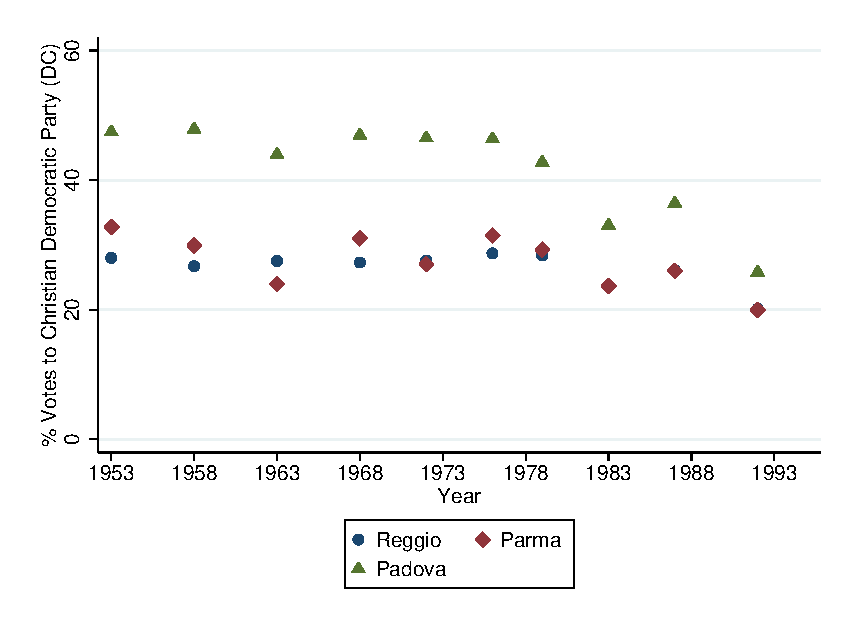
\includegraphics[width=\textwidth]{../../output/image/DC.eps}
\caption{Christian Democrats}
        \end{subfigure}
        \begin{subfigure}[t]{0.49\textwidth}
          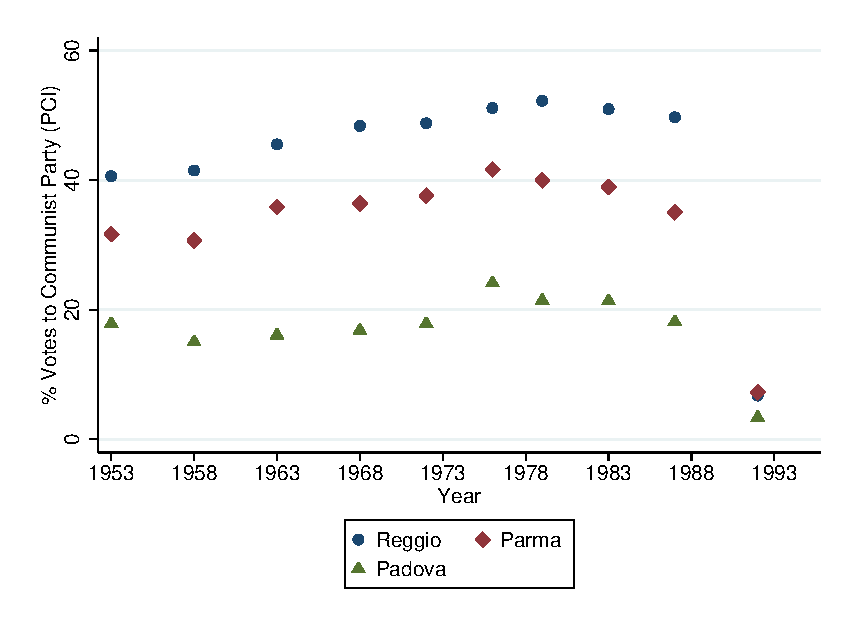
\includegraphics[width=\textwidth]{../../output/image/PCI.eps}
 \caption{Communist Party}
        \end{subfigure}
      \caption{Election Statistics}  \label{fig:election}
    \end{figure}

    \begin{figure}[H]
    \centering
    \caption{Religious Marriages}
    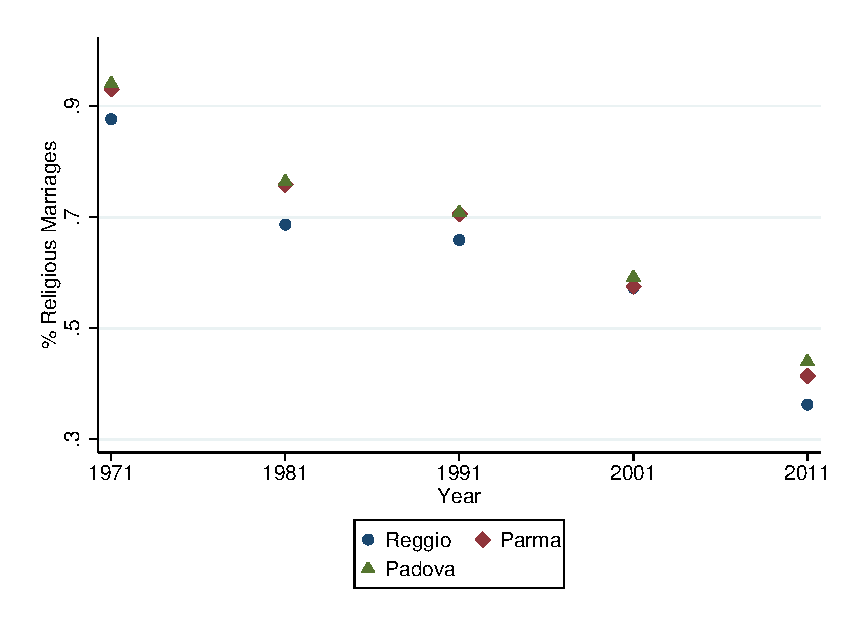
\includegraphics[width=\textwidth]{../../output/rel_mar.eps}
	\end{figure}
	
\begin{figure}[H]
      \centering
        \begin{subfigure}[t]{0.49\textwidth}
          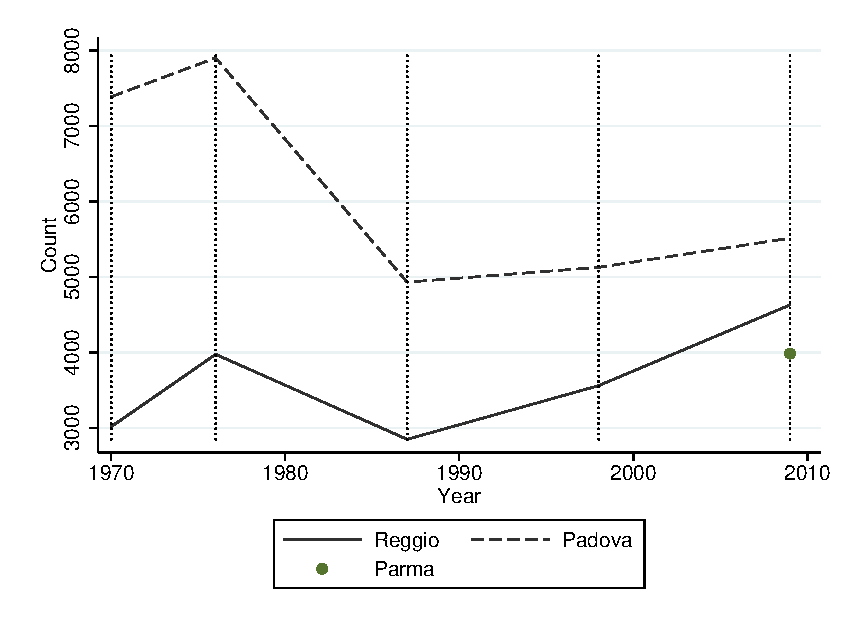
\includegraphics[width=\textwidth]{../../output/image/enroll_num_graph.eps}
\caption{Num. of Children Enrolled in Preschool}
        \end{subfigure}
        \begin{subfigure}[t]{0.49\textwidth}
          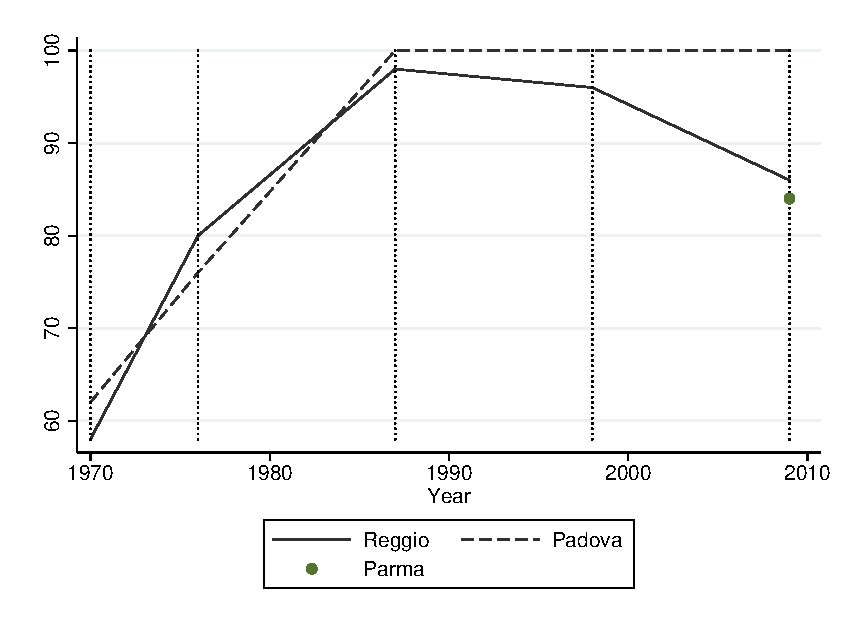
\includegraphics[width=\textwidth]{../../output/image/enroll_per_graph.eps}
 \caption{Percentage of Ages 3-5 Enrolled in Preschool}
        \end{subfigure}
        \begin{subfigure}[t]{0.49\textwidth}
          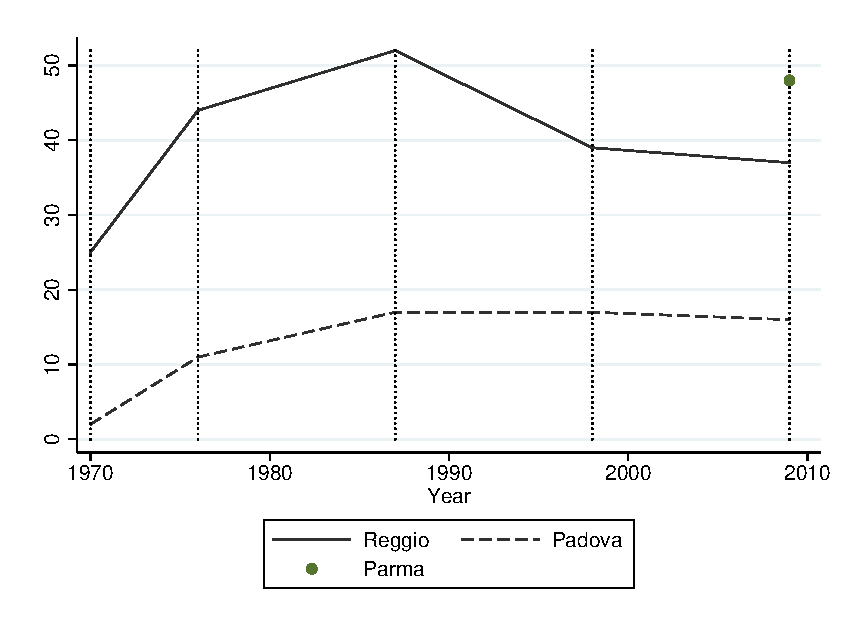
\includegraphics[width=\textwidth]{../../output/image/enroll_per_muni_graph.eps}
        \caption{Percentage of Enrollment in Municipal Preschools}
        \end{subfigure}
        \begin{subfigure}[t]{0.49\textwidth}
          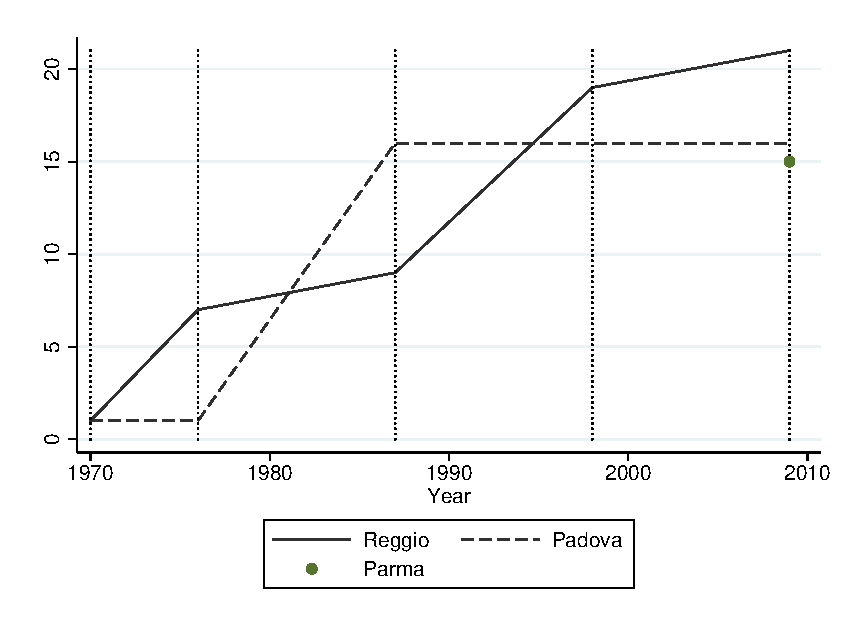
\includegraphics[width=\textwidth]{../../output/image/enroll_per_stat_graph.eps}
            \caption{Percentage of Enrollment in State Preschools}
        \end{subfigure}
      \begin{subfigure}[ht]{0.48\textwidth}
        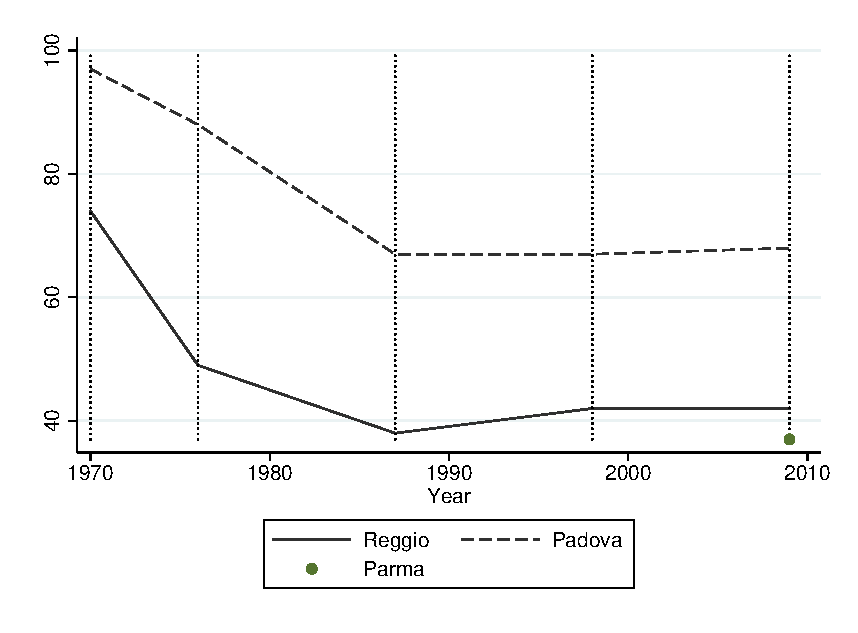
\includegraphics[width=\textwidth]{../../output/image/enroll_per_priv_graph.eps}
        \caption{Percentage of Enrollment in Religious Preschools}
        \label{fig:large}
      \end{subfigure}
      \caption{Enrollment Statistics}  \label{fig:enrollment}
    \end{figure}    